\begin{figure*}[t]
\centering
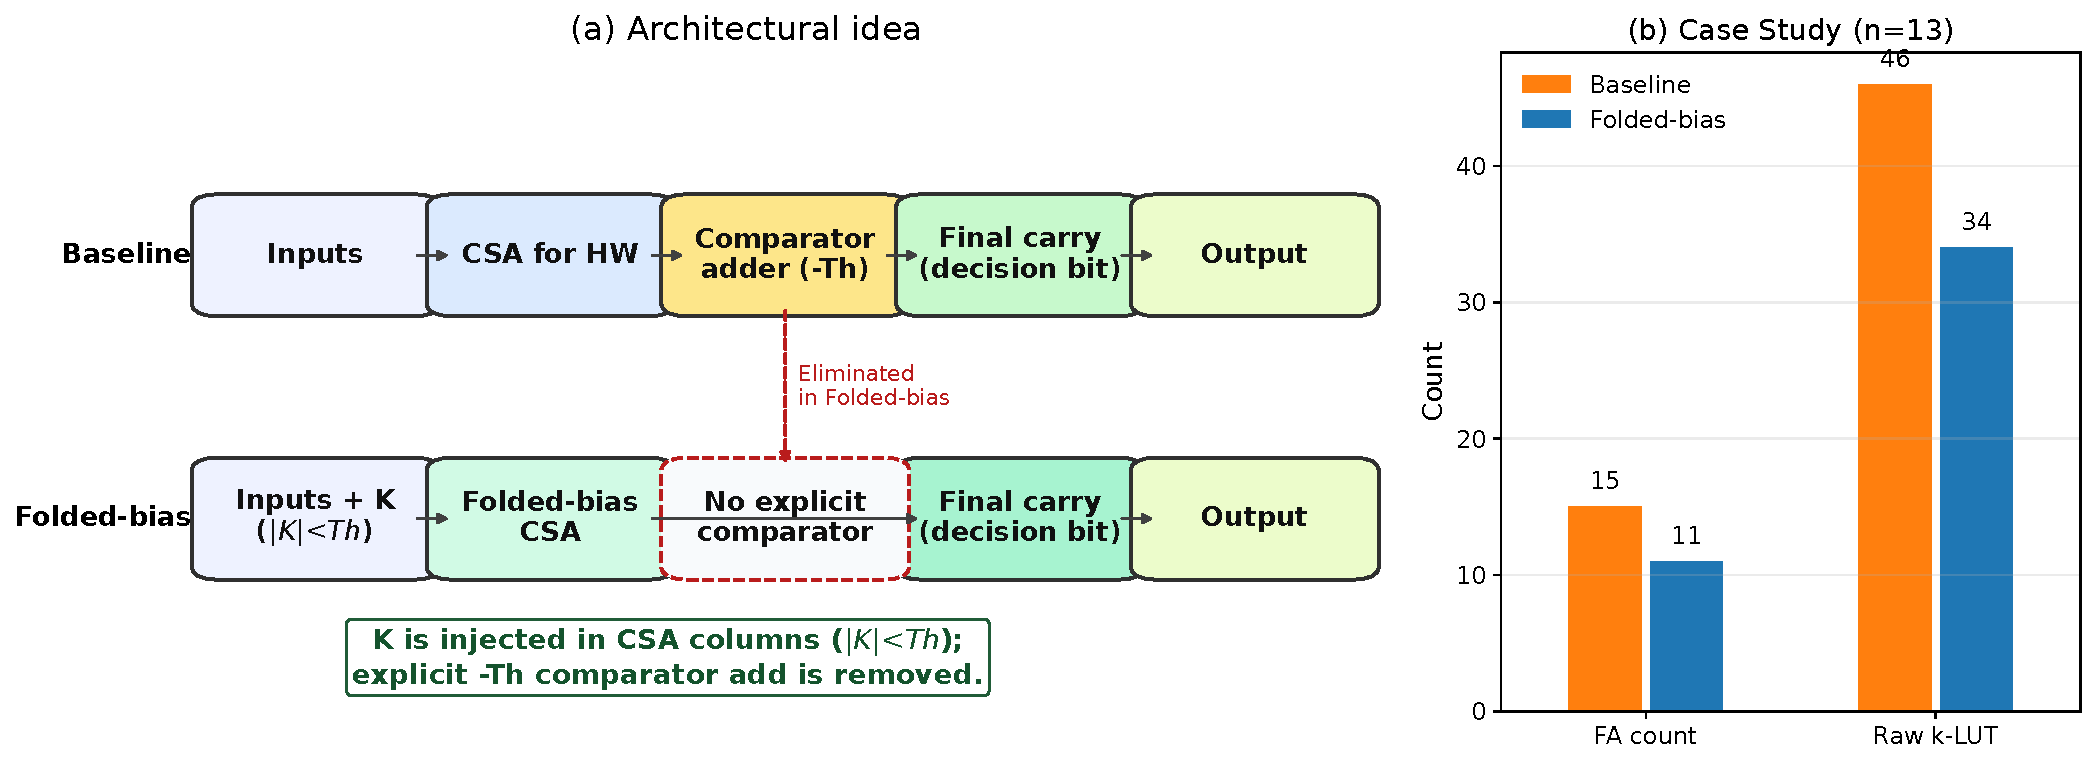
\includegraphics[width=\textwidth]{results/paper_package_5_61/figures/fig_intro_motivation.pdf}
\caption{Introduction-level motivation for folded-bias decomposition. (a) Baseline computes HW with CSA, performs an explicit comparator add with $-Th$, and then derives the final carry decision bit. Folded-bias injects $K$ directly into CSA columns and derives the same decision bit without a separate comparator stage. (b) Example at $n=13$: FA count reduces by $\Delta$FA=4 (26.7\%), and raw $k$-LUT structural size reduces by $\Delta$raw-$k$-LUT=12 (26.1\%) versus baseline.}
\label{fig:intro_motivation}
\end{figure*}
